\DiaryEntry{Primality Tests}{2021-04-06}{Number Theory}

\subsection{Fermat Test}

This on is based on Fermat's theorem; see \ref{2020-12-09:entry}.

\begin{theorem}
    let $p$ be a prime and suppose $p \nmid a$. Then

    \bee
        a^{p-1} \equiv 1 \mod p
    \eee
\end{theorem}

The simplest version is to chose a \emph{base} $a$, calculate $a^{n-1} \mod n$ for our prime candidate $n$ and check whether it equals $1$. The caveat is, that Fermat's theorem works only one way; i.e. there exist \emph{pseudoprimes in base $a$} which are composite numbers but for which 

\bee
    a^{n-1} \equiv 1 \mod n
\eee

holds nevertheless. The solution to that is to repeat the calculation of $a^{n-1} \mod n$ for various bases $a$.

\begin{verbatim}
    Repeat k times:
        Pick a randomly in the range [2;n-2]
        If a^(n-1) mod n != 1:
            return "composite"
    return "probably prime"
\end{verbatim}

The larger $k$ is, the less likely it is to hit a pseudoprime (to all tried bases) and the smaller the likelyhood for a false positive becomes.

We next count the number of pseudoprimes a given number has. This is done in the script \href{https://github.com/ClemensFMN/JuliaStuff/blob/master/NumberTheory/pseudo_primes.jl}{here}. In the following Figure we plot the number of pseudoprimes as function of \emph{composite} $n$.

\begin{figure}[H]
    \centering
    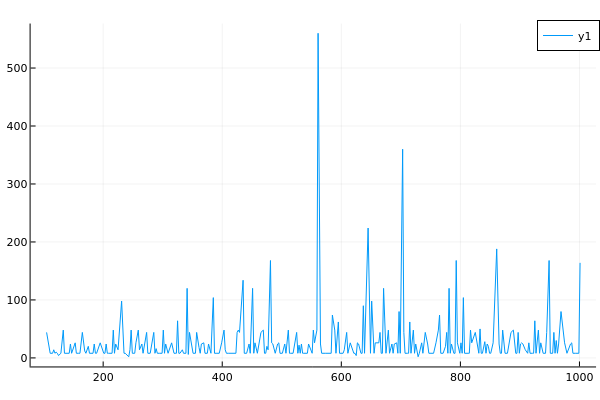
\includegraphics[scale=0.6]{images/2021-04-06-pseudo_primes_1.png}
\end{figure}


Wee see that the number of pseudoprimes is mostly well below $50$; however, there are certain outliers which have more pseudoprimes. The most striking one is at $n=561$ which is actually the smallest Carmichael number, but there are others as well; e.g. $n = 703$ has about $400$ pseudoprimes. If we would use a small $k$ in above primality test algorithm, there wold be a large chance that we chose only pseudoprimes as basis and concluded that $703$ would be prime.

There is also a slightly plot with a larger range from $1001$ to $5001$ wich shows a similar behaviour.

\begin{figure}[H]
    \centering
    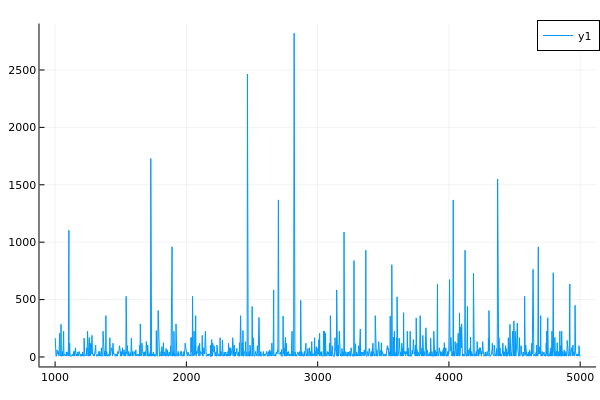
\includegraphics[scale=0.6]{images/2021-04-06-pseudo_primes_2.png}
\end{figure}

The problem is that there are infinitely many Carmichael numbers; they are less dense than prime numbers but there are so many that Fermat's primality test is usually not used.

\subsection{Miller–Rabin Primality Test}



%%% Local Variables:
%%% mode: latex
%%% TeX-master: "journal"
%%% End:
